\section{性能测试对比}
针对上述对SM4加密算法性能的7种优化方案,分别在7种不同输入数据规模(1 KB至16 MB)下测试程序的运行时间并计算吞吐率与加速比,过程截图如下:
\begin{figure}[H]
    \centering
    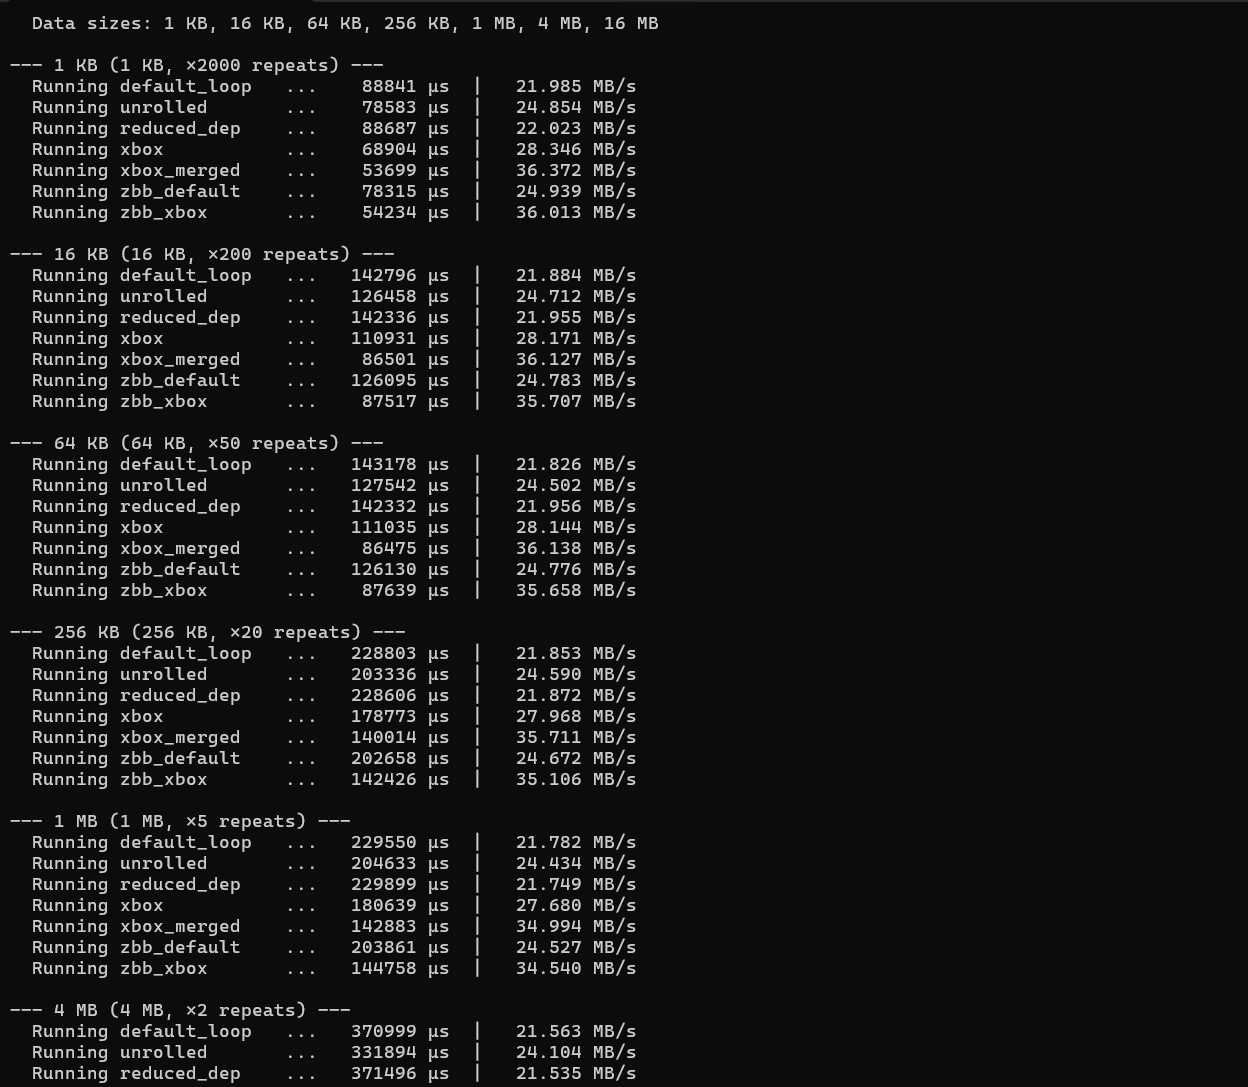
\includegraphics[width = 1\textwidth]{figure/more_test_data.png}
    \caption{对比测试各种优化方案效率}
\end{figure}

以默认循环实现(\texttt{default\_loop})为基准,所有方案在每个数据规模下的运行时间(elapsed\_us)、吞吐率(throughput\_mbps)和加速比(speedup)数据汇总如下。

% ===== 表1: 运行时间 =====
\begin{table}[H]
\centering
\caption{各方案在不同数据规模下的运行时间 (单位: $\mu$s)}
\label{tab:elapsed}
\begin{tabular}{l|c|c|c|c|c|c|c}
\toprule
\textbf{数据规模} & \multicolumn{7}{c}{\textbf{运行时间 (elapsed\_us)}} \\
\cline{2-8}
& default\_loop & unrolled & reduced\_dep & xbox & xbox\_merged & zbb\_default & zbb\_xbox \\
\midrule
1 KB      & 88,841 & 78,583 & 88,687 & 68,904 & 53,699 & 78,315 & 54,234 \\
16 KB     & 142,796 & 126,458 & 142,336 & 110,931 & 86,501 & 126,095 & 87,517 \\
64 KB     & 143,178 & 127,542 & 142,332 & 111,035 & 86,475 & 126,130 & 87,639 \\
256 KB    & 228,803 & 203,336 & 228,606 & 178,773 & 140,014 & 202,658 & 142,426 \\
1 MB      & 229,550 & 204,633 & 229,899 & 180,639 & 142,883 & 203,861 & 144,758 \\
4 MB      & 370,999 & 331,894 & 371,496 & 293,106 & 236,653 & 329,914 & 239,037 \\
16 MB     & 753,325 & 675,472 & 753,503 & 600,482 & 493,941 & 671,899 & 500,540 \\
\bottomrule
\end{tabular}
\end{table}

% ===== 表2: 吞吐率 =====
\begin{table}[H]
\centering
\caption{各方案在不同数据规模下的吞吐率 (单位: MB/s)}
\label{tab:throughput}
\begin{tabular}{l|c|c|c|c|c|c|c}
\toprule
\textbf{数据规模} & \multicolumn{7}{c}{\textbf{吞吐率 (throughput\_mbps)}} \\
\cline{2-8}
& default\_loop & unrolled & reduced\_dep & xbox & xbox\_merged & zbb\_default & zbb\_xbox \\
\midrule
1 KB      & 21.985 & 24.854 & 22.023 & 28.346 & 36.372 & 24.939 & 36.013 \\
16 KB     & 21.884 & 24.712 & 21.955 & 28.171 & 36.127 & 24.783 & 35.707 \\
64 KB     & 21.826 & 24.502 & 21.956 & 28.144 & 36.138 & 24.776 & 35.658 \\
256 KB    & 21.853 & 24.590 & 21.872 & 27.968 & 35.711 & 24.672 & 35.106 \\
1 MB      & 21.782 & 24.434 & 21.749 & 27.680 & 34.994 & 24.527 & 34.540 \\
4 MB      & 21.563 & 24.104 & 21.535 & 27.294 & 33.805 & 24.249 & 33.468 \\
16 MB     & 21.239 & 23.687 & 21.234 & 26.645 & 32.393 & 23.813 & 31.965 \\
\bottomrule
\end{tabular}
\end{table}

% ===== 表3: 加速比 =====
\begin{table}[H]
\centering
\caption{各方案在不同数据规模下的加速比 (基准: default\_loop)}
\label{tab:speedup}
\begin{tabular}{l|c|c|c|c|c|c}
\toprule
\textbf{数据规模} & \multicolumn{6}{c}{\textbf{加速比 (speedup, $\times$ vs baseline)}} \\
\cline{2-7}
& unrolled & reduced\_dep & xbox & xbox\_merged & zbb\_default & zbb\_xbox \\
\midrule
1 KB      & 1.1305 & 1.0017 & 1.2893 & 1.6544 & 1.1344 & 1.6381 \\
16 KB     & 1.1292 & 1.0032 & 1.2873 & 1.6508 & 1.1324 & 1.6316 \\
64 KB     & 1.1226 & 1.0059 & 1.2895 & 1.6557 & 1.1352 & 1.6337 \\
256 KB    & 1.1252 & 1.0009 & 1.2799 & 1.6341 & 1.1290 & 1.6065 \\
1 MB      & 1.1218 & 0.9985 & 1.2708 & 1.6066 & 1.1260 & 1.5858 \\
4 MB      & 1.1178 & 0.9987 & 1.2658 & 1.5677 & 1.1245 & 1.5521 \\
16 MB     & 1.1153 & 0.9998 & 1.2545 & 1.5251 & 1.1212 & 1.5050 \\
\bottomrule
\end{tabular}
\end{table}